\chapter{Phương pháp tìm kiếm địa phương}
\label{chap:search}

Như đã trình bày trong chương \ref{chap:solution}, hầu hết các thuật toán hiện đại đều dựa trên tìm kiếm địa phương và thuộc lớp cải tiến. Thuật toán không cố gắng để đưa ra ngay một nghiệm tối ưu ngay từ đầu (hay chỉ với một bước chạy). Thay vào đó, ta xuất phát từ một nghiệm chấp nhận được (thường được khởi tạo nhanh như thuật toán tham lam chẳng hạn), sau đó qua mỗi bước lặp, nghiệm được cải thiện dần cho đến khi điều kiện dừng được thỏa mãn. Tại mỗi bước lặp, thuật toán cố gắng khám phá không gian nghiệm bằng cách xét các lân cận của nghiệm hiện tại để tìm một nghiệm tối ưu địa phương. 

Chiến thuật này cần ta định nghĩa rõ ràng khái niệm "lân cận", "tối ưu địa phương", "tiêu chí chấp nhận nghiệm" và "điều kiện dừng". Lân cận được hiểu là tập hợp các nghiệm chấp nhận được (theo nghĩa thỏa mãn các ràng buộc) với một thay đổi không quá lớn từ nghiệm hiện tại. Ví dụ, một vài yêu cầu từ tuyến này được tráo đổi với tuyến khác hoặc được chuyển hẳn sang một tuyến khác hay là tạo một tuyến mới. Nghiệm tối ưu địa phương là nghiệm tốt nhất ta có thể tìm được trong lân cận như vậy. Tuy nhiên, nếu ta tiếp tục tìm kiếm từ nghiệm tối ưu địa phương thì đôi khi thuật toán bị "mắc" tại nghiệm đó. Cụ thể hơn, thuật toán trải qua nhiều bước lặp mà chỉ xét các nghiệm lân cận của một tối ưu địa phương hoặc độ cải thiện là rất chậm. Chính vì vậy, có nhiều tiêu chí chấp nhận hay tiêu chí lựa chọn nghiệm để thuật toán thoát khỏi vùng này được phát triển thay vì chỉ chấp nhận nghiệm có chi phí nhỏ nhất trong lân cận. Một vài tiêu chí có thể kể đến như \textit{tìm kiếm tabu} (\textit{tabu search}), \textit{mô phỏng luyện kim} (\textit{simulated annealing}), \textit{chấp nhận với ngưỡng} (\textit{threshold-accepting}) hay \textit{duyệt qua bản ghi} (\textit{record-to-record travel}) đã được trình bày ở chương trước. Nhìn chung, thay vì tiếp tục tìm kiếm từ một tối ưu địa phương, chúng ta đưa vào hàm mục tiêu một hệ số phạt (nhỏ) nào đó để có thể tìm kiếm từ một nghiệm tệ hơn nghiệm tối ưu địa phương một chút. Điều kiện dừng thường được áp dụng là số bước lặp tối đa hoặc thời gian tối đa mà thuật toán được phép chạy. Thời gian này thường được gọi là \textit{timeout}.

\section{Tìm kiếm lân cận rộng}
\section{Tìm kiếm lân cận rộng thích ứng}
Tìm kiếm lân cận rộng thích ứng (\textit{adaptive large neighbourhood search - ALNS}) được giới thiệu bởi S. Ropke và D. Pisinger \cite{ropke2006adaptive} là một mở rộng của LNS. Thay vì chỉ sử dụng một chiến thuật hủy và một chiến thuật thêm lại yêu cầu như LNS, ALNS cho phép lựa chọn nhiều toán tử hủy và thêm lại. Việc này cho phép thuật toán tìm kiếm không gian nghiệm một cách linh hoạt hơn và khó bị bẫy ở một nghiệm tối ưu cục bộ. Điểm thú vị của ALNS là các thuật toán hủy và thêm lại không được chọn một cách ngẫu nhiên mà lựa chọn có trọng số phụ thuộc vào trạng thái (nghiệm hiện tại) của bài toán.

\subsection{Lựa chọn phương pháp xóa và thêm lại}
Để lựa chọn phương pháp xóa và thêm lại, ta gán cho mỗi heuristic một trọng số khác nhau và sử dụng nguyên tắc "bánh xe lựa chọn". Nếu có $k$ heuristic với trọng số $w_i, i \in \{1,...,k\}$, ta chọn heuristic $j$ với xác suất
\begin{equation}
	\label{eq:select}
	p_j = \frac{w_j}{\sum_{i=1}^k w_i}.
\end{equation}
Lưu ý rằng, việc lựa chọn thuật toán xóa và thêm lại là độc lập với nhau. Các trọng số này có thể được thiết lập thủ công và không đổi trong suốt vòng đời của việc tìm kiếm hoặc nó có thể được điều chỉnh tự động để "thích ứng" với trạng thái hiện tại của hệ. Một cách điều chỉnh các tham số này tự động được trình bày ngay sau đây.

\subsection{Điều chỉnh tham số tự động}
Trọng số được điều chỉnh mỗi khi có nghiệm mới được chấp nhận. Ý tưởng chung là theo dõi một điểm số đại diện cho độ hiệu quả của thuật toán trong các vòng lặp gần đây. Điểm số càng cao thì thuật toán được chọn càng hiệu quả. Quá trình tìm kiếm được chia thành nhiều bước, mỗi bước là một số vòng lặp. Điểm của mỗi heuristic được đặt là $0$ khi bắt đầu và được tăng thêm $\sigma_1, \sigma_2, \sigma_3$ tùy thuộc vào tình huống.
\begin{table}[caption={Tham số cập nhật trọng số.}, label=tab:weight]
	\begin{tabularx}{\textwidth}{|l|X|}
		\hline
		Tham số    & Mô tả  \\ \hline
		$\sigma_1$ & Hành động xóa-chèn cuối cùng dẫn đến một nghiệm mới tốt hơn nghiệm tốt nhất toàn cục. \\ \hline
		$\sigma_2$ & Hành động xóa-chèn cuối cùng dẫn đến một nghiệm mới có chi phí tốt hơn chi phí của nghiệm hiện tại. \\ \hline
		$\sigma_3$ & Hành động xóa-chèn cuối cùng dẫn đến một nghiệm mới có chi phí tệ hơn chi phí của nghiệm hiện tại nhưng thỏa mãn điều kiện chấp nhận nghiệm. \\ \hline
	\end{tabularx}
\end{table}

Trong mỗi bước, thao tác xóa và thêm lại được cập nhật một lượng như nhau vì ta không chắc sự "cải thiện" nghiệm đến từ việc xóa hay thêm lại yêu cầu. Mỗi khi kết thúc bước, ta tính toán lại trọng số mới sử dụng các điểm số trên. Gọi $\omega_{ij}$ là trọng số của heuristic $i$ trong bước $j$. Ta đánh các trọng số như nhau tại bước đầu tiên, sau đó khi bước $j$ kết thúc, ta tính lại trọng số cho tất cả các heuristic để sử dụng cho bước $j+1$ như sau
\begin{equation}
	\label{eq:adaptive_weight}
	\omega_{i, j+1} = \omega_{ij}(1-r)+r\frac{\pi_i}{\theta_i}.
\end{equation}
Trong đó $\pi_i$ là điểm số của heuristic $i$ trong bước $j$ và $\theta_i$ là số lần ta cố gắng sử dụng heuristic $i$ trong bước $j$. Tham số $r$ là tham số điều khiển tốc độ điều chỉnh trọng số (được đặt mặc định bằng $0.1$ trong thực nghiệm). Nếu $r=0$, nghĩa là chúng ta không sử dụng điểm để điều chỉnh trọng số hay nói cách khác là các trọng số được giữ nguyên từ trong suốt quá trình tìm kiếm. Nếu $r=1$, nghĩa là ta lấy điểm thu được từ bước gần nhất để quyết định trọng số.

Việc điều chỉnh trọng số như trên làm tăng xác suất chọn thuật toán xóa (chèn) đã mang lại hiệu quả ở bước trước đó. Về cơ bản, với việc sử dụng chiến thuật điều chỉnh trọng số như trên, ta kì vọng rằng các thuật toán xóa (chèn) đã hiệu quả ở bước trước thì cũng sẽ hiệu quả ở bước tiếp theo. Trong thực nghiệm, các tham số được lựa chọn lần lượt là $\sigma_1=10$, $\sigma_2=4$ và $\sigma_3=2$.

\subsection{Thêm nhiễu khi chỉnh tham số tự động}
Như đã trình bày, với việc sử dụng chiến thuật lựa chọn tham số tự động như trên, ta kì vọng rằng thuật toán nếu đang hiệu quả thì nó sẽ tiếp tục hiệu quả. Tuy nhiên việc cộng một lượng cố định vào thuật toán đó về lâu dài (khi trải qua nhiều vòng lặp) thì trọng số của nó trở lên lớn dẫn đến xác suất lựa chọn thuật toán này cũng lớn theo. Chúng ta cũng chưa sử dụng yếu tố vòng lặp (hay thời gian chạy). Do đó, tác giả đề xuất ý tưởng đơn giản là nếu rất "lâu" rồi ta mới có một thuật toán hiệu quả thì ta cũng nên điều chỉnh trọng số của nó theo "thời gian chờ đó". Giả sử sau $m$ vòng lặp, chúng ta mới lại có một nghiệm được chấp nhận từ lần cuối cùng nghiệm được chấp nhận, trọng số của thuật toán sẽ được điều chỉnh một lượng tỉ lệ với $1 - e^{-\gamma m}$. Hàm $\text{exp}$ được sử dụng để chuẩn hóa lượng này trong khoảng $(0,1)$ khi $m$ lớn hoặc nhỏ. Cuối cùng ta có biểu thức cho trọng số của thuật toán như sau
\begin{equation}
	\label{eq:boost_adaptive_weight}
	\omega_{i, j+1} = \omega_{ij}(1-r)+r\frac{\pi_i} {\theta_i} + \alpha \beta (1 - e^{-\gamma m})
\end{equation}
với $\alpha$ (có thể âm hoặc dương) và $\gamma$ (dương) là các tham số điều khiển, $\beta$ là một số ngẫu nhiên trong khoảng $(0,1)$ \footnote[1]{Trong thực nghiệm, các tham số được đặt mặc định $\alpha = -1$, $\gamma = 1$. Ta có thể điều chỉnh các tham số này tùy thuộc vào bài toán để thu được kết quả tốt nhất.}. Trong phần thực nghiệm \ref{sec:performance}, tác giả sẽ chỉ ra sự vượt trội về hiệu năng khi thêm nhiễu vào việc điều chỉnh trọng số như trên. Chính vì vậy, thuật toán được đặt tên là B-ALNS (\textit{Boosted - Adaptive Large Neighborhood Search}).

\subsection{Số lượng yêu cầu bỏ đi và thêm lại}
\label{sec:num_rm_req}
Số lượng yêu cầu bỏ đi và thêm lại trong mỗi vòng lặp là một tham số quan trọng. Nếu số lượng yêu cầu bỏ đi và thêm lại quá ít, thuật toán sẽ không thể khám phá được không gian nghiệm một cách đủ lớn. Nếu số lượng yêu cầu bỏ đi và thêm lại quá nhiều, thuật toán sẽ tốn nhiều thời gian tính toán và không thể tìm được nghiệm tốt trong thời gian hợp lý. Việc lựa chọn một con số phù hợp với kích thước của cấu hình (đầu vào) và tài nguyên của máy tính không đơn giản. Trong thực nghiệm, tác giả đã thử nghiệm với nhiều con số khác nhau và nhận thấy rằng, việc sử dụng một lượng yêu cầu bỏ đi và thêm lại ngẫu nhiên trong một khoảng nhất định (phụ thuộc vào kích thước cấu hình) thu được chất lượng nghiệm cũng như hiệu năng tổng thể tốt hơn so với việc chỉ sử dụng một con số cố định. Số yêu cầu được bỏ đi thường không vượt quá $10\%$ kích thước cấu hình theo D. Pisinger và S. Ropke \cite{pisinger2007general}. Đối với các cấu hình kích thước lớn, số lượng yêu cầu bỏ đi nằm trong khoảng từ 30 đến 60.
\chapter{Ứng dụng ALNS vào CVRPTW}

\begin{figure}[H] % places figure environment here   
  \centering % Centers Graphic
  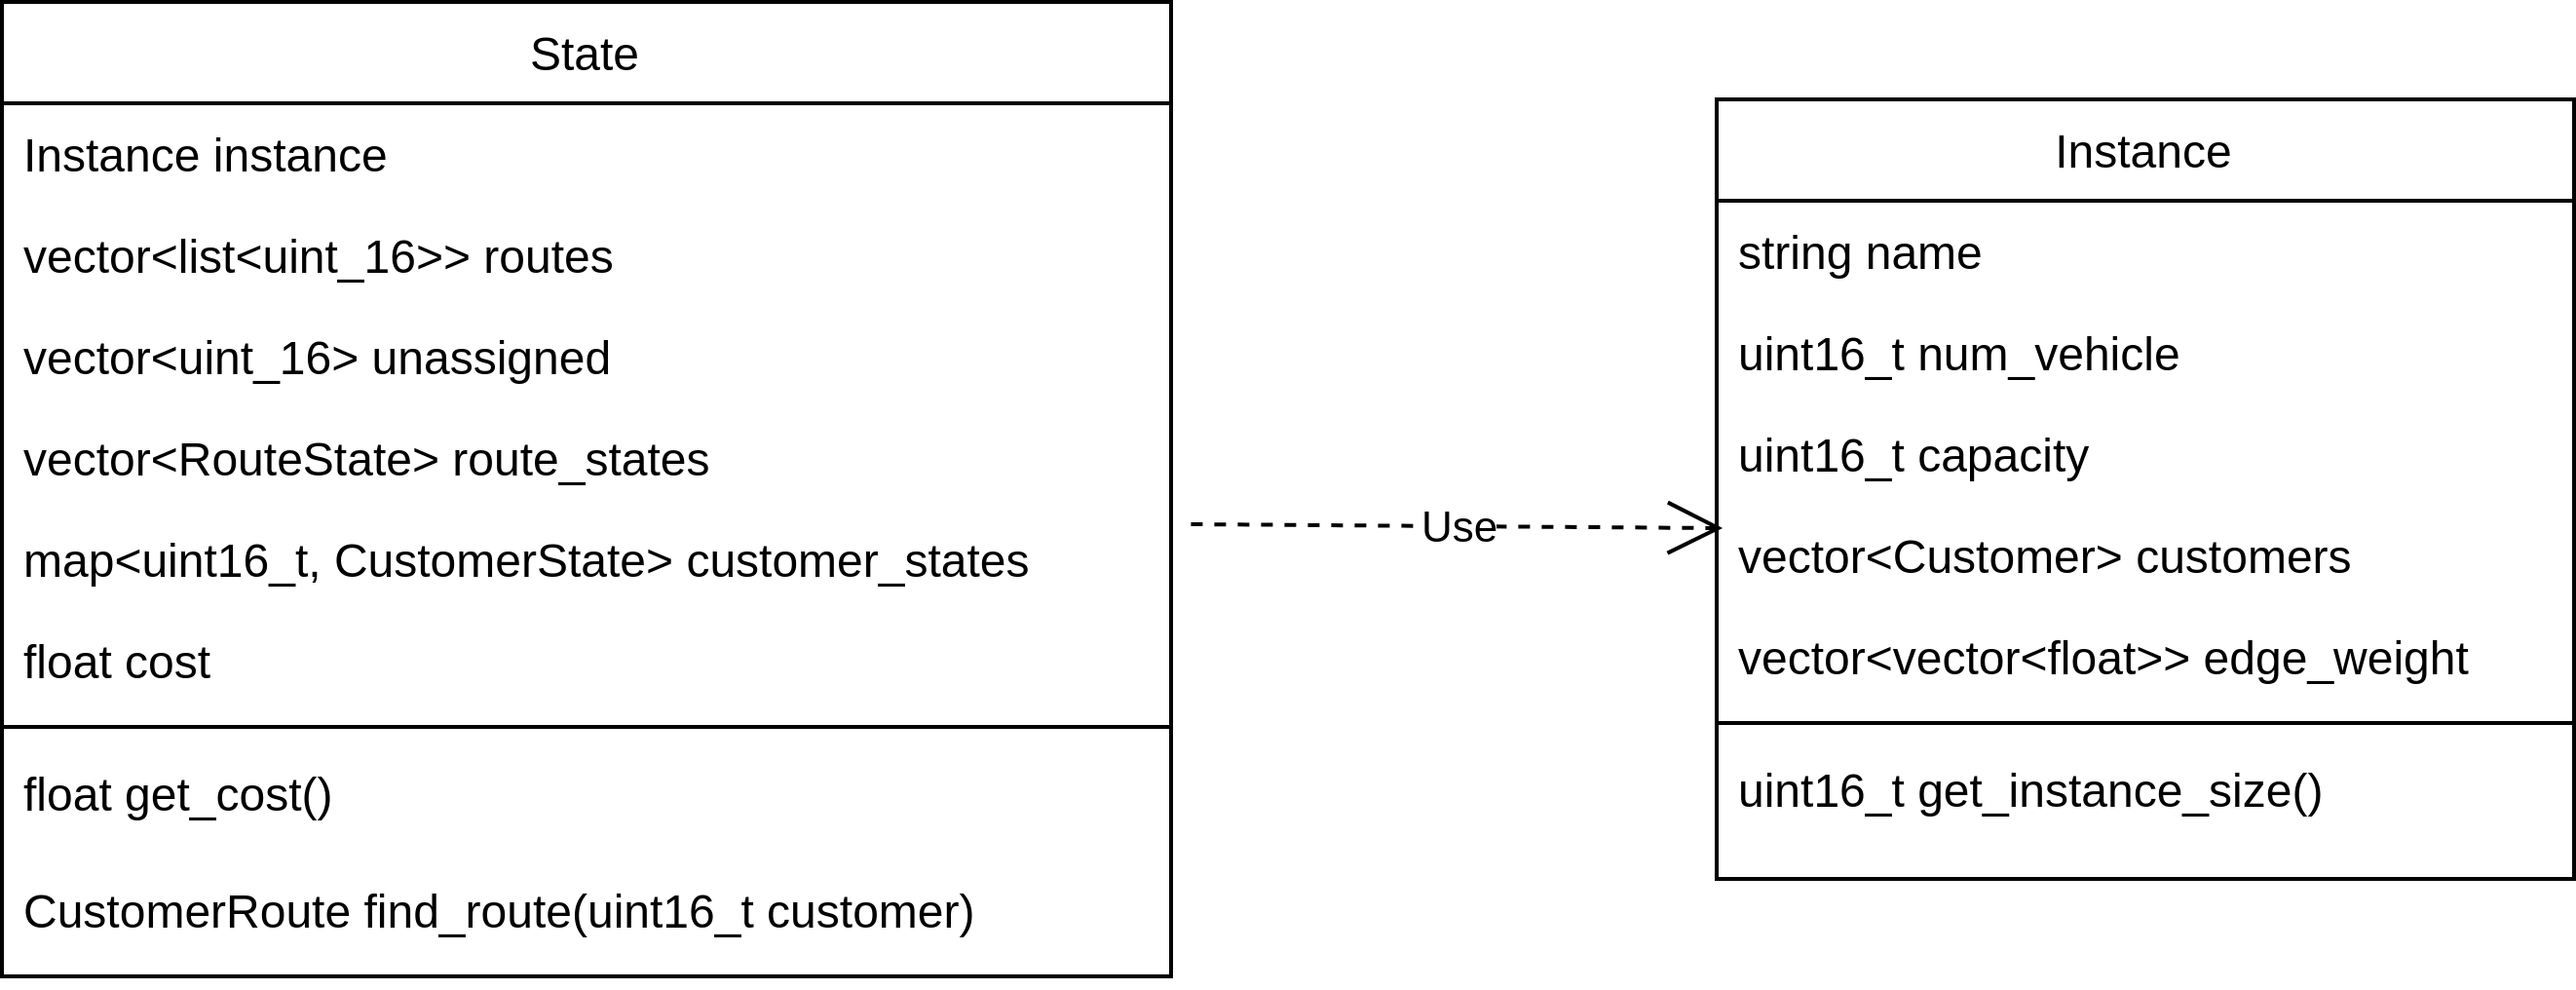
\includegraphics[width=1\textwidth]{figures/core-object.png} 
  % \includesvg[scale=1]{figures/core-object}
  \caption{Đối tượng chính của chương trình} 
  \label{fig:fg_02}
\end{figure}